\begin{figure}
  \centering
  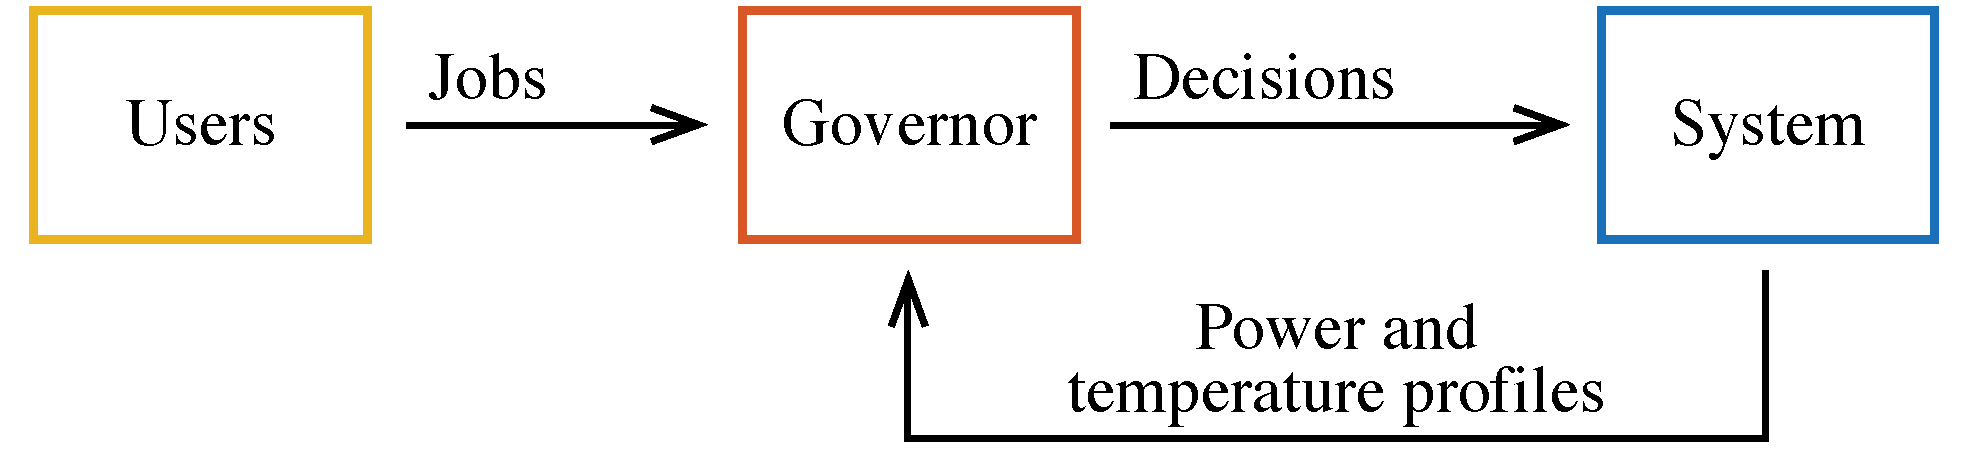
\includegraphics[width=1.0\columnwidth]{include/assets/figures/usage.pdf}
  \caption{A usage example with a feedback loop.}
  \flab{usage}
\end{figure}

Our vision of the primary usage of the methodology was emphasized multiple times
in Sec.~\ref{sec:introduction}--\ref{sec:problem-formulation}. However, after
having the methodology and toolchain presented in \sref{methodology} and
\sref{toolchain}, we would like to give some more intuition. In this section, we
shall dive deeper into the internals of the Streamer module in
\fref{methodology} and Main module in \fref{streamer}.

As noted in \sref{composition} and \sref{streamer}, a scheduling or, more
generally, management policy is assumed by the Streamer module. Conceiving and
developing such a policy based on learning from the data available on the chip
is the main application of the work presented in this paper. From this
perspective, the methodology can be viewed as a provider of a highly responsive
infrastructure or environment around the policy. Figure~\ref{fig:usage}
illustrates this standpoint, in which the policy is referred to as ``Governor.''
The Governor module is, in a sense, extraneous to us whereas the modules to the
left and right from it are in our jurisdiction. More concretely, the generation
of a stream of jobs is an imitation of a user behavior, which we try to
replicate as realistically as possible by using reference data. On the other
hand, the synthesis of power and temperature profiles is an imitation of the
response of the underlying platform to the incoming user requests and the
actions taken by the governor. In this scenario, the management policy is
assumed to learn from the data and perfect itself accordingly, which is
emphasized in \fref{usage} by a feedback from the Platform module to the
Governor module. In real life, this feedback is readings of various hardware
sensors and software counters.

There is another scenario that we would like to mention separately, and it is a
special case of the one described above. Assure now that there is no feedback
from Platform to Governor in \fref{usage}. In this case, the pipeline serves the
sole purpose of generating data. These data can be stored and used for
developing techniques for the prediction of power and temperature in an abstract
setting, that is, without any specific or, perhaps, with many diverse
applications in mind.
